\documentclass[9pt]{beamer}
\usepackage[utf8]{}
\usepackage[]{babel}
\usetheme{Rochester}
\usepackage{graphicx}
\setbeamercolor{structure}{fg=blue!300!black}
\usepackage{multicol}
\usepackage{cite} 
\usepackage{hyperref}
\usepackage{titletoc}
\usepackage{graphicx}
\usepackage{color} 
\usecolortheme{seahorse}
\usepackage{amsmath, amsfonts, amssymb, amsxtra, amsthm, bm}
\usepackage{mathrsfs}
\usepackage{dsfont}
\usepackage{verbatim}
\usepackage{soulutf8}
\usepackage{comment}
\usepackage{booktabs}
\usepackage[framemethod=TikZ]{mdframed}
\usepackage{mathdots}
\usepackage{bm}
\setcounter{MaxMatrixCols}{15}
\usepackage{array}
\usepackage{bbm}
\newtheorem{conjecture}[theorem]{Conjecture}
\newtheorem{corollary}
\newtheorem{lemma}
\newtheorem{rmk}{Remark}
\setbeamertemplate{footline}[frame number]

\newcommand{\F}{\mathbb{F}}
\newcommand{\N}{\mathbb{N}}
\newcommand{\Z}{\mathbb{Z}}
\newcommand{\Q}{\mathbb{Q}}
\newcommand{\R}{\mathbb{R}}
\usepackage[
backend=biber,
style=authortitle,
sorting=none
]{biblatex}
\addbibresource{references.bib}

\title[]{The VC Dimension of Dudley-Like Classes Over Real-Valued Polynomials}
\author[]{James Hanby, Tran Duy Anh Le, Rohan Soni, Maxwell Sun, and Jake Wellington}
\institute{Tripods/Stemforall 2022}


\begin{document}
\nocite{*}
\frame{\titlepage}  % trang bìa

\AtBeginSection{
\begin{frame}{Table of Contents}
  \tableofcontents[currentsection]
\end{frame}
}
\section{Introduction}
\subsection{Introduction to VC Dimension}
\begin{frame}{Definition}
\begin{definition}
    Let $X$ be a set. We define the \textbf{hypothesis collection} of functions
    $$\mathcal{H}: X \rightarrow \{0,1 \}$$
    A set $S \subset X$ is \textbf{shattered} by $\mathcal{H}$ if for any subset $S'$ of $S$, there exists a function $h \in \mathcal{H}$ such that
    $$h(x) = \begin{cases}
    1 & \text{If $x \in S'$}\\
    0 & \text{If $x \not \in S'$}\\
    \end{cases}$$
    \pause
    The \textbf{VC Dimension} of $\mathcal{H}$ is the size of the largest shattered set. We denote it as $VCDim(\mathcal{H})$. Notice that this value might be infinity as $\mathcal{H}$ may shatter sets with any size.
\end{definition}
\pause
\begin{example}
Example: Consider $X$ to be the set of real numbers. We defined the hypothesis class to be
$$\mathcal{H} = \{\mathbbm{1}_{[a,b]}: -\infty < a < b < \infty \}$$
Then $VCDim(\mathcal{H}) = 2$
% \begin{itemize}
%     \item
%     \begin{equation*}
%         (a+b)c=ab+bc\mod p
%     \end{equation*}
%     \item
% \end{itemize}
\end{example}
\end{frame}
% \begin{frame}{Introduction (Continue)}

% \begin{itemize}
%     \item Firstly, we show that $\mathcal{H}$ can shatter $2$ points. Consider $S=\{0,2 \}$, then we will have
%     \begin{center}
%     \begin{tabular}{ | c | c | c |} 
%     \hline
%     h(x) & h(0) & h(2)\\ 
%     \hline
%     $\mathbbm{1}_{[0.5,5]}(x)$ & 0 & 0\\
%     \hline
%     $\mathbbm{1}_{[-1,3]}(x)$ & 1 & 1\\
%     \hline
%     $\mathbbm{1}_{[1,3]}(x)$ & 0 & 1\\
%     \hline
%     $\mathbbm{1}_{[-1,1]}(x)$ & 1 & 0\\
%     \hline
%     \end{tabular}
%     \end{center}
%     \pause
%     \item Hence, $\mathcal{H}$ can shatter $2$ points. Hence, $VCDim(\mathcal{H}) \geq 2$\\
%     \pause
%     \item Now, we will show that it cannot shattered $3$ points. Suppose not, if $\mathcal{H}$ can shattered $S=\{x_1,x_2,x_3\}$ with $x_1<x_2<x_3$. Then there exists $h=\mathbbm{1}_{[a,b]} \in \mathcal{H}$ such that
%     $$h(x_1)=h(x_3)=1,h(x_2)=0$$
%     \pause
%     \item However, we will have $a<x_1<x_2<x_3<b$, which shows that $h(x_2)=1$, a contradiction\\
%     \pause
%     \item Hence, $VCDim(\mathcal{H}) \leq 2$ or we must have $VCDim(\mathcal{H})$
% \end{itemize}


% \end{frame}

\subsection{Dudley class}
\begin{frame}{Dudley Classes}
\begin{definition}
Let $F$ be a finite dimensional subspace of functions $X \rightarrow \mathbb{R}$. Take
$$\mathcal{H} = \{\mathbbm{1}_{\geq 0} \circ f| f \in F \}$$
Then $VCDim(H)=Dim \ F$. This is called a \textbf{Dudley Class}.
\end{definition}
\pause
\vskip.3in
\begin{example}
% Take $F = \text{span} \{x^2+y^2,x,y,1 \}$. Then $VCDim(\mathcal{H})=4$
Take $F$ to be the set of linear functionals on $\mathbb{R}^n$. Then $\mathcal{H}$ is the set of indicator functions of halfspaces in $\mathbb{R}^n$ with the origin on the boundary. I.e.
$$F = \{x \mapsto a \cdot x| a \in \mathbb{R}^n\}$$
and
$$\mathcal{H} = \{\mathbbm{1}_S| S = \{x| a \cdot x \ge 0\} \text{ for some } a \in \mathbb{R}^n\}$$
$\mathcal{H}$ then has VC dimension $\dim F = n$.
\end{example}
\end{frame}
\section{Application to Learning Theory}
\begin{frame}{How Does This Apply?}
    \begin{itemize}
        \item Situation: there is a function we are trying to predict that maps elements of $X$ to $0$ or $1$.
        \vskip.3in
        \pause
        \item We are given access to finitely many randomly chosen samples from $X$ and their associated correct labels.
        \vskip.30in
        \pause
    \end{itemize}
    \begin{definition}
    We say that a class $\mathcal{H}$ of functions $X \rightarrow \{0,1\}$ is $\textbf{probably}$ $\textbf{approximately}$ $\textbf{learnable}$ (or PAC learnable) if there exists a learning algorithm that can predict any function $f\in \mathcal{H}$ with at most $\epsilon$ error and probability at least $1 - \delta$, given access to labeled random samples of $X$.
    \end{definition}
\end{frame}
\begin{frame}{How Does This Apply? (Continued)}
    \begin{theorem} [Fundamental Theorem of Statistical Learning]
    If $\mathcal{H}$ has VC dimension $d$, then $\mathcal{H}$ is PAC learnable if and only if $d$ is finite. Specifically, if the number of required samples to ensure this is $m$, then
    $$
    C_1 \frac{d + \log(1/\delta)}{\epsilon} \le m \le C_2 \frac{d \log(1/\epsilon) + \log(1/\delta)}{\epsilon}
    $$
    where $C_1$ and $C_2$ are absolute constants.
    \end{theorem}
\end{frame}
\begin{frame}{How Does This Apply? (Continued)}
    \begin{itemize}
        \vskip.25in
        \item In our case, the learning problem is predicting a function from
        $$
        \mathcal{H} = \{\mathbbm{1}_{\mathbb{Q}} \circ f|\text{ f is a polynomial of max degree }n\}
        $$
        \pause
        \vskip.35in
        \item As you will see, the conjecture implies that the number of samples needed to be probably approximately correct is finite.
    \end{itemize}
\end{frame}
\section{Main Theorem}
\subsection{Theorem 1}
\begin{frame}{Theorem}
\begin{itemize}
    \item From the definition of a Dudley Class, what if we change from considering $\geq 0$ to some other field?\\
    \pause
    \vskip.2in
    \item Considering this, we have the following conjecture:
\end{itemize}

\pause
\vskip.20in
\begin{conjecture}
Suppose $X$ is the set of real numbers and $F=\text{span}\{1,x,\cdots,x^n\}$. We define the hypothesis class $\mathcal{H}$ to be
$$\mathcal{H} = \{\mathbbm{1}_{\mathbb{Q}} \circ f| f \in F \}$$
Then we will have $VCDim(\mathcal{H}) = 2dim \ F -1$
\end{conjecture}
\end{frame}

\subsection{Examples and illustrations}
\begin{frame}{The case $n=0$}
\begin{itemize}
    \item Consider the case $Dim \ F = 1$. We have $f(x) = c$ for some constant $c$. The following figure shows that $\mathcal{H}$ shatters $1$ point:
\end{itemize}

\pause
\begin{figure}
        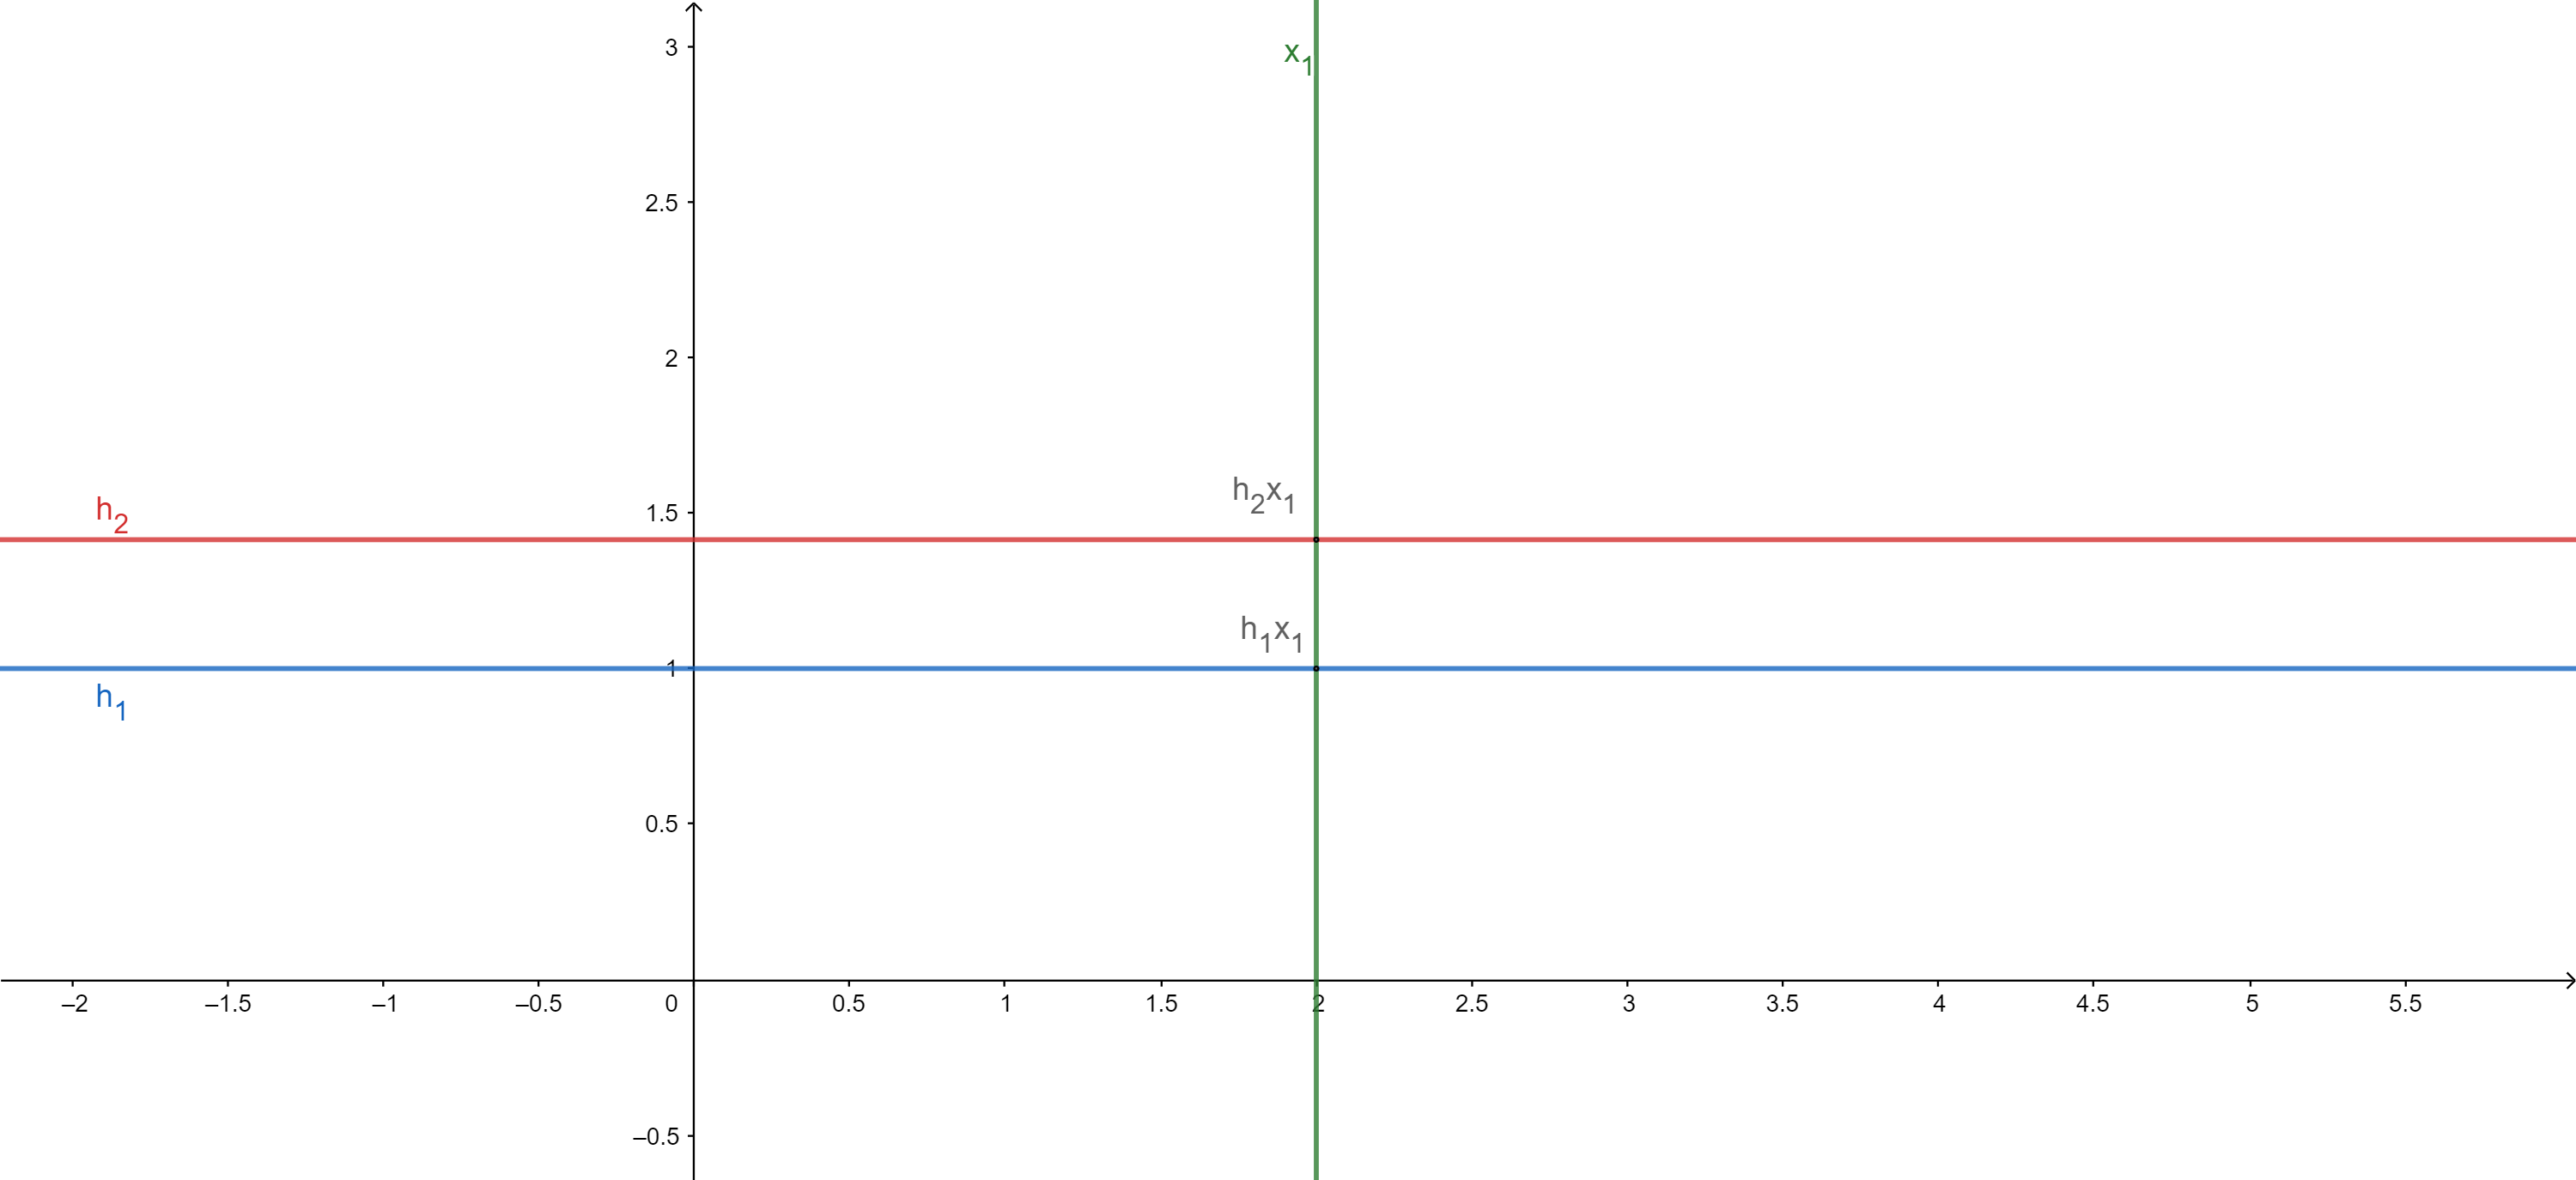
\includegraphics[width = 1 \linewidth]{geogebra-export (1).png}
        \caption{The case $n=0$, with $x_1=1, h_1(x)=1,h_2(x)=\sqrt{2}$}
        \label{fig:my_label}
\end{figure}
\end{frame}
\begin{frame}{The case $n=1$}
\begin{itemize}
    \item Consider the case $Dim \ F = 2$, where we are dealing with functions $f(x) = ax+b$ for some constants $a,b$. 
    \pause
    \item Consider the set $S=\{1,\sqrt{2},1+\sqrt{2} \}$. 
    \pause
    \item We have the following functions for proof that $S$ is shattered:
\end{itemize}

\begin{center}
\begin{tabular}{ | c | c | c | c |} 
\hline
h(x) & h(1) & h(\sqrt{2}) & h(1+\sqrt{2})\\ 
\hline
$h_1(x) = \mathbbm{1}_{\mathbb{Q}} \circ 1$ & 1 & 1 & 1\\
\hline
$h_2(x) =  \mathbbm{1}_{\mathbb{Q}} \circ \sqrt{2}$ & 0 & 0 & 0\\
\hline
$h_3(x) = \mathbbm{1}_{\mathbb{Q}} \circ \frac{2}{3}x$ & 1 & 0 & 0\\
\hline
$h_4(x) = \mathbbm{1}_{\mathbb{Q}} \circ (\sqrt{2}x)$ & 0 & 1 & 0\\
\hline
$h_5(x) = \mathbbm{1}_{\mathbb{Q}} \circ ((1-\sqrt{2})x)$ & 0 & 0 & 1\\
\hline
$h_6(x) = \mathbbm{1}_{\mathbb{Q}} \circ ((1+\sqrt{2})x-\sqrt{2})$ & 1 & 1 & 0\\
\hline
$h_7(x) = \mathbbm{1}_{\mathbb{Q}} \circ (\sqrt{2}x-\sqrt{2})$ & 1 & 0 & 1\\
\hline
$h_8(x) = \mathbbm{1}_{\mathbb{Q}} \circ (x-\sqrt{2})$ & 0 & 1 & 1\\
\hline
\end{tabular}
\end{center}

\end{frame}
\begin{frame}{The case $n=1$ (Continued)}
\begin{itemize}
    \item The following figure shows these functions in a graph:
\end{itemize}
\pause
\begin{figure}
        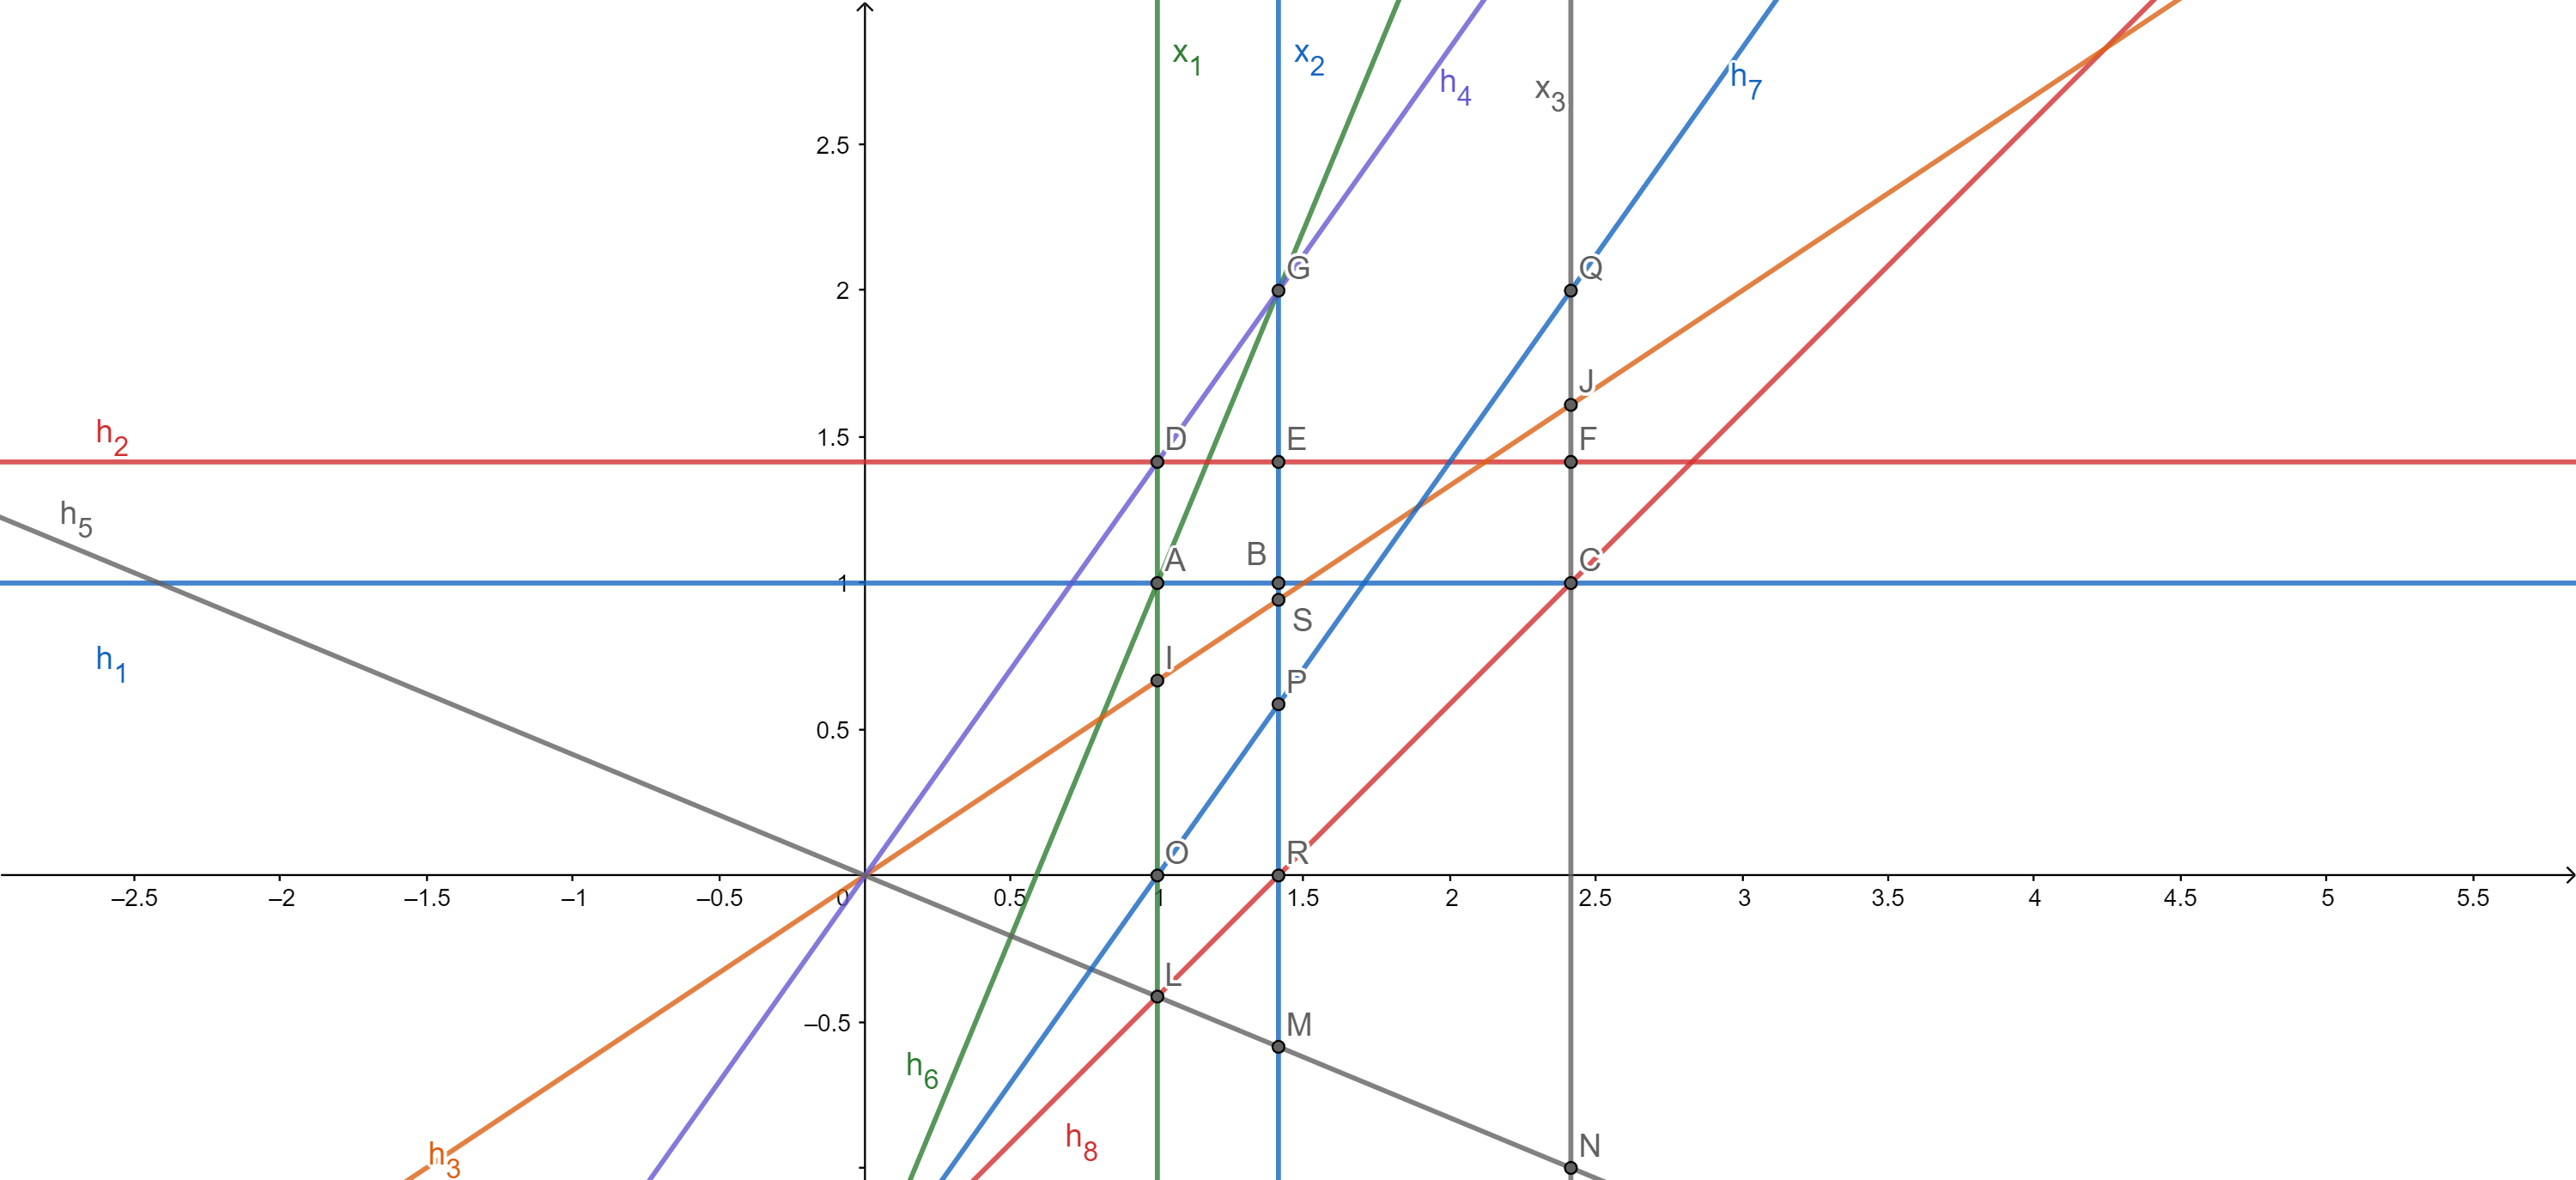
\includegraphics[width = 1 \linewidth]{geogebra-export (3).png}
        \caption{The case $\mathcal{H}$ shatters $3$ points}
        \label{fig:my_label}
\end{figure}
\end{frame}

\begin{frame}{The case $n=1$ (Continued)}
    
    \begin{itemize}
        \item We show $VCDim(\mathcal{H}) \leq 3$. 
        \vskip.25in
        \pause
        \item Suppose $\mathcal{H}$ can shatter $4$ points $x_1,x_2,x_3,x_4$. Then consider $h_1(x) = a_1x+b_1$ such that
        $$h_1(x_1)=h_1(x_2)=h_1(x_3) = 1, h_1(x_4)=0$$
        \pause
        \item From that, we get $a_1 \neq 0$. Then  $a_1(x_3-x_1), a_1(x_2-x_1) \in \mathbb{Q}$. Hence, 
        $$\frac{x_3-x_1}{x_2-x_1} \in \mathbb{Q}$$
    \end{itemize}
\end{frame}
\begin{frame}{The case $n=1$ (Continued)}
\begin{itemize}
    \item Let $c=x_2-x_1$. Then $x_3-x_1 = cq_1$ for some rational number $q_1 \neq 0$. 
    \pause
    \vskip.4in
    \item By a similar argument, we can also show $x_4-x_1 = cq_2$ for some rational number $q_2 \neq 0$. 
    \vskip.4in
    \item We wish to reach a contradiction by showing that $h_1(x_4)$ is rational
    
\end{itemize}
\end{frame}
\begin{frame}{The case $n=1$ (Continued)}
\begin{itemize}
    \item We have
    \begin{align*}
        h_1(x_4) &= a_1(cq_2+x_1)+b_1 \\
        &= a_1cq_2+a_1x_1+b_1 \\
        &= \frac{q_2}{q_1} (a_1cq_1)+a_1x_1+b_1 \\
        &= \frac{q_2}{q_2} (a_1(x_3-x_1)) + h_1(x_1) \\
        &= \frac{q_2}{q_2}(h_1(x_3)-h_1(x_1)) + h_1(x_1) \in \mathbb{Q}
    \end{align*}
    \pause
    \item This is a contradiction, since $h_1$ was defined so that $h_1(x_4)$ is irrational.
    \pause
    \vskip.2in
    \item Hence, $VCDim(\mathcal{H}) \leq 3$
\end{itemize}
\end{frame}

\section{Proof of the main theorem}
\subsection{Case n=2}
\begin{frame}{Proof that when $n=2$, $VCDim(\mathcal{H}) \geq 5$}
    \begin{itemize}
        \item To begin with, we state a key theorem required for this case:
        \pause
    \end{itemize}
    \vskip.5in
    \begin{Theorem}[Lagrange Interpolation Formula]
    Let $x_1,x_2,\cdots,x_{n+1}$ be distinct reals and $y_1,y_2,\cdots,y_{n+1}$ be any real numbers. There exists a unique polynomial $P(x)$ with degree at most $n$ such that $P(x_i)=y_i$ for all $i$. $P$ is given by
    $$P(x) = \displaystyle \sum_{i=1}^{n+1} y_i \frac{\displaystyle \prod_{j \neq i} (x-x_j)}{\displaystyle \prod_{j \neq i} (x_i-x_j)}$$
    \end{Theorem}
    % \pause
    % \begin{proof}
    % Consider $Q(x) = \displaystyle \sum_{i=1}^{n+1} y_i \frac{\displaystyle \prod_{j \neq i} (x-x_j)}{\displaystyle \prod_{j \neq i} (x_i-x_j)}$ and let $R(x) = P(x)-Q(x)$. Then we have $\deg P, \deg Q, \deg R \leq n$. However, we have
    % $$R(x_i) = P(x_i)-Q(x_i) = y_i - y_i =0 \ \forall 1 \leq i \leq n+1$$
    % Therefore, we have $R(x) \equiv 0$ or $P(x) = Q(x)$
    % \end{proof}
\end{frame}

\begin{frame}{Proof that when $n=2$, $VCDim(\mathcal{H}) \geq 5$ (Continued)}
\begin{itemize}
    \item We choose $x_1=1,x_2=2+\sqrt{2},x_3=3-\sqrt{2},x_4=4+2\sqrt{2},x_5=5-2\sqrt{2}$ and we show that $\mathcal{H}$ can shatter these points. Call this set $S$\\
    \pause
    \vskip.40in
    \item The case that $\mathcal{H}$ shatters any subset of these points of size $0, 1, 2$, or $5$ is easy to prove.
    \vskip.40in
    \pause
    \item We just need to focus on the case $\mathcal{H}$ shatters $3$ or $4$ points\\
\end{itemize}
\end{frame}
\begin{frame}{Proof that when $n=2$, $VCDim(\mathcal{H}) \geq 5$ (Continued)}
\begin{itemize}
    \item By Lagrange Interpolation formula, we have that for any distinct $i,j,k$,
    $$f(x) = f(x_i)\frac{(x-x_j)(x-x_k)}{(x_i-x_j)(x_i-x_k)}+f(x_j)\frac{(x-x_i)(x-x_k)}{(x_j-x_i)(x_j-x_k)}+f(x_k)\frac{(x-x_i)(x-x_j)}{(x_k-x_i)(x_k-x_j)}$$
    \pause
    \vskip.50in
    \item Let $T(x,x_i,x_j,x_k)$ denote $\frac{(x-x_i)(x-x_j)}{(x_k-x_i)(x_k-x_j)}$. We will calculate different values of $T$ depending on what subset of $S$ we wish to realize.
\end{itemize}
\end{frame}
\begin{frame}{Prove that when $n=2$, $VCDim(\mathcal{H}) \geq 5$ (Continue)}
    \begin{itemize}
        \item For example, consider the case where $f(x_1),f(x_2),f(x_3) \in \mathbb{Q}$. With some calculations, we will have\\
        \begin{center}
        \begin{tabular}{ | c | c |} 
        \hline
        $T(x_4,x_1,x_2,x_3) $ & $\frac{-65}{7}+\frac{-46}{7}\sqrt{2}$\\
        \hline
        $T(x_4,x_2,x_3,x_1) $ & $-7+4\sqrt{2}$\\
        \hline
        $T(x_4,x_3,x_1,x_2) $ & $\frac{23}{7}+\frac{18}{7}\sqrt{2}$\\
        \hline
        $T(x_5,x_1,x_2,x_3) $ & $\frac{18}{7}+\frac{-6}{7}\sqrt{2}$\\
        \hline
        $T(x_5,x_2,x_3,x_1) $ & $-9+6\sqrt{2}$\\
        \hline
        $T(x_5,x_3,x_1,x_2) $ & $\frac{52}{7}+\frac{-36}{7}\sqrt{2}$\\
        \hline
        \end{tabular}
        \end{center}
        \pause
        \vskip.3in
        \item The idea is to choose the values of $f(x_1),f(x_2),f(x_3) \in \mathbb{Q}$ based on if we want to make $f(x_4),f(x_5)$ rational or not. There will be $3$ cases.
    \end{itemize}
\end{frame}
\begin{frame}{Proof that when $n=2$, $VCDim(\mathcal{H}) \geq 5$ (Continued)}
\begin{itemize}
    \item Case 1: If $f(x_4) \in \mathbb{Q},f(x_5) \not \in \mathbb{Q}$, then by looking at the coefficient of $\sqrt(2)$ in our interpolation expression, we obtain the system of equations
    $$\begin{cases}
    4f(x_1)+\frac{18}{7}f(x_2)+\frac{-46}{7}f(x_3) = 0\\
    6f(x_1)+\frac{-36}{7}f(x_2)+\frac{-6}{7}f(x_3) \neq 0
    \end{cases}$$
    Take $f(x_1)=\frac{1}{14},f(x_2)=\frac{-1}{9},f(x_3)=0$, we will have the polynomial $f_{30}(x)$ satisfy the condition that $f(x_1),f(x_2),\cdots,f(x_4) \in \mathbb{Q}$, while $f(x_5) \not \in \mathbb{Q}$
    \pause
    \vskip.2in
    \item Case 2: If $f(x_4) \not \in \mathbb{Q},f(x_5) \in \mathbb{Q}$, then take $f(x_1)=\frac{1}{7},f(x_2)=\frac{1}{6},f(x_3)=0$. We get the polynomial $f_{30}(x)$ satisfying the condition that $f(x_1),f(x_2),\cdots,f(x_5) \in \mathbb{Q}$, while $f(x_4) \not \in \mathbb{Q}$
    \pause
    \vskip.2in
    \item Case 3: If $f(x_4) \not \in \mathbb{Q},f(x_5) \not \in \mathbb{Q}$, then take the sum of the previous polynomials will get the result
\end{itemize}
\end{frame}
\begin{frame}{Prove that when $n=2$, $VCDim(\mathcal{H}) \geq 5$ (Continue)}
    \begin{itemize}
        \item With the same idea as above, we can construct $32$ polynomials $f_0(x),f_1(x),\cdots,f_{31}(x)$ that satisfy
        $$f_i(x_j) = 1 \iff \text{In the binary representation of $i$, the $j^{th}$ number will be $1$}$$
        \pause
        \item Here is the image of the graphs :)
        \begin{figure}
        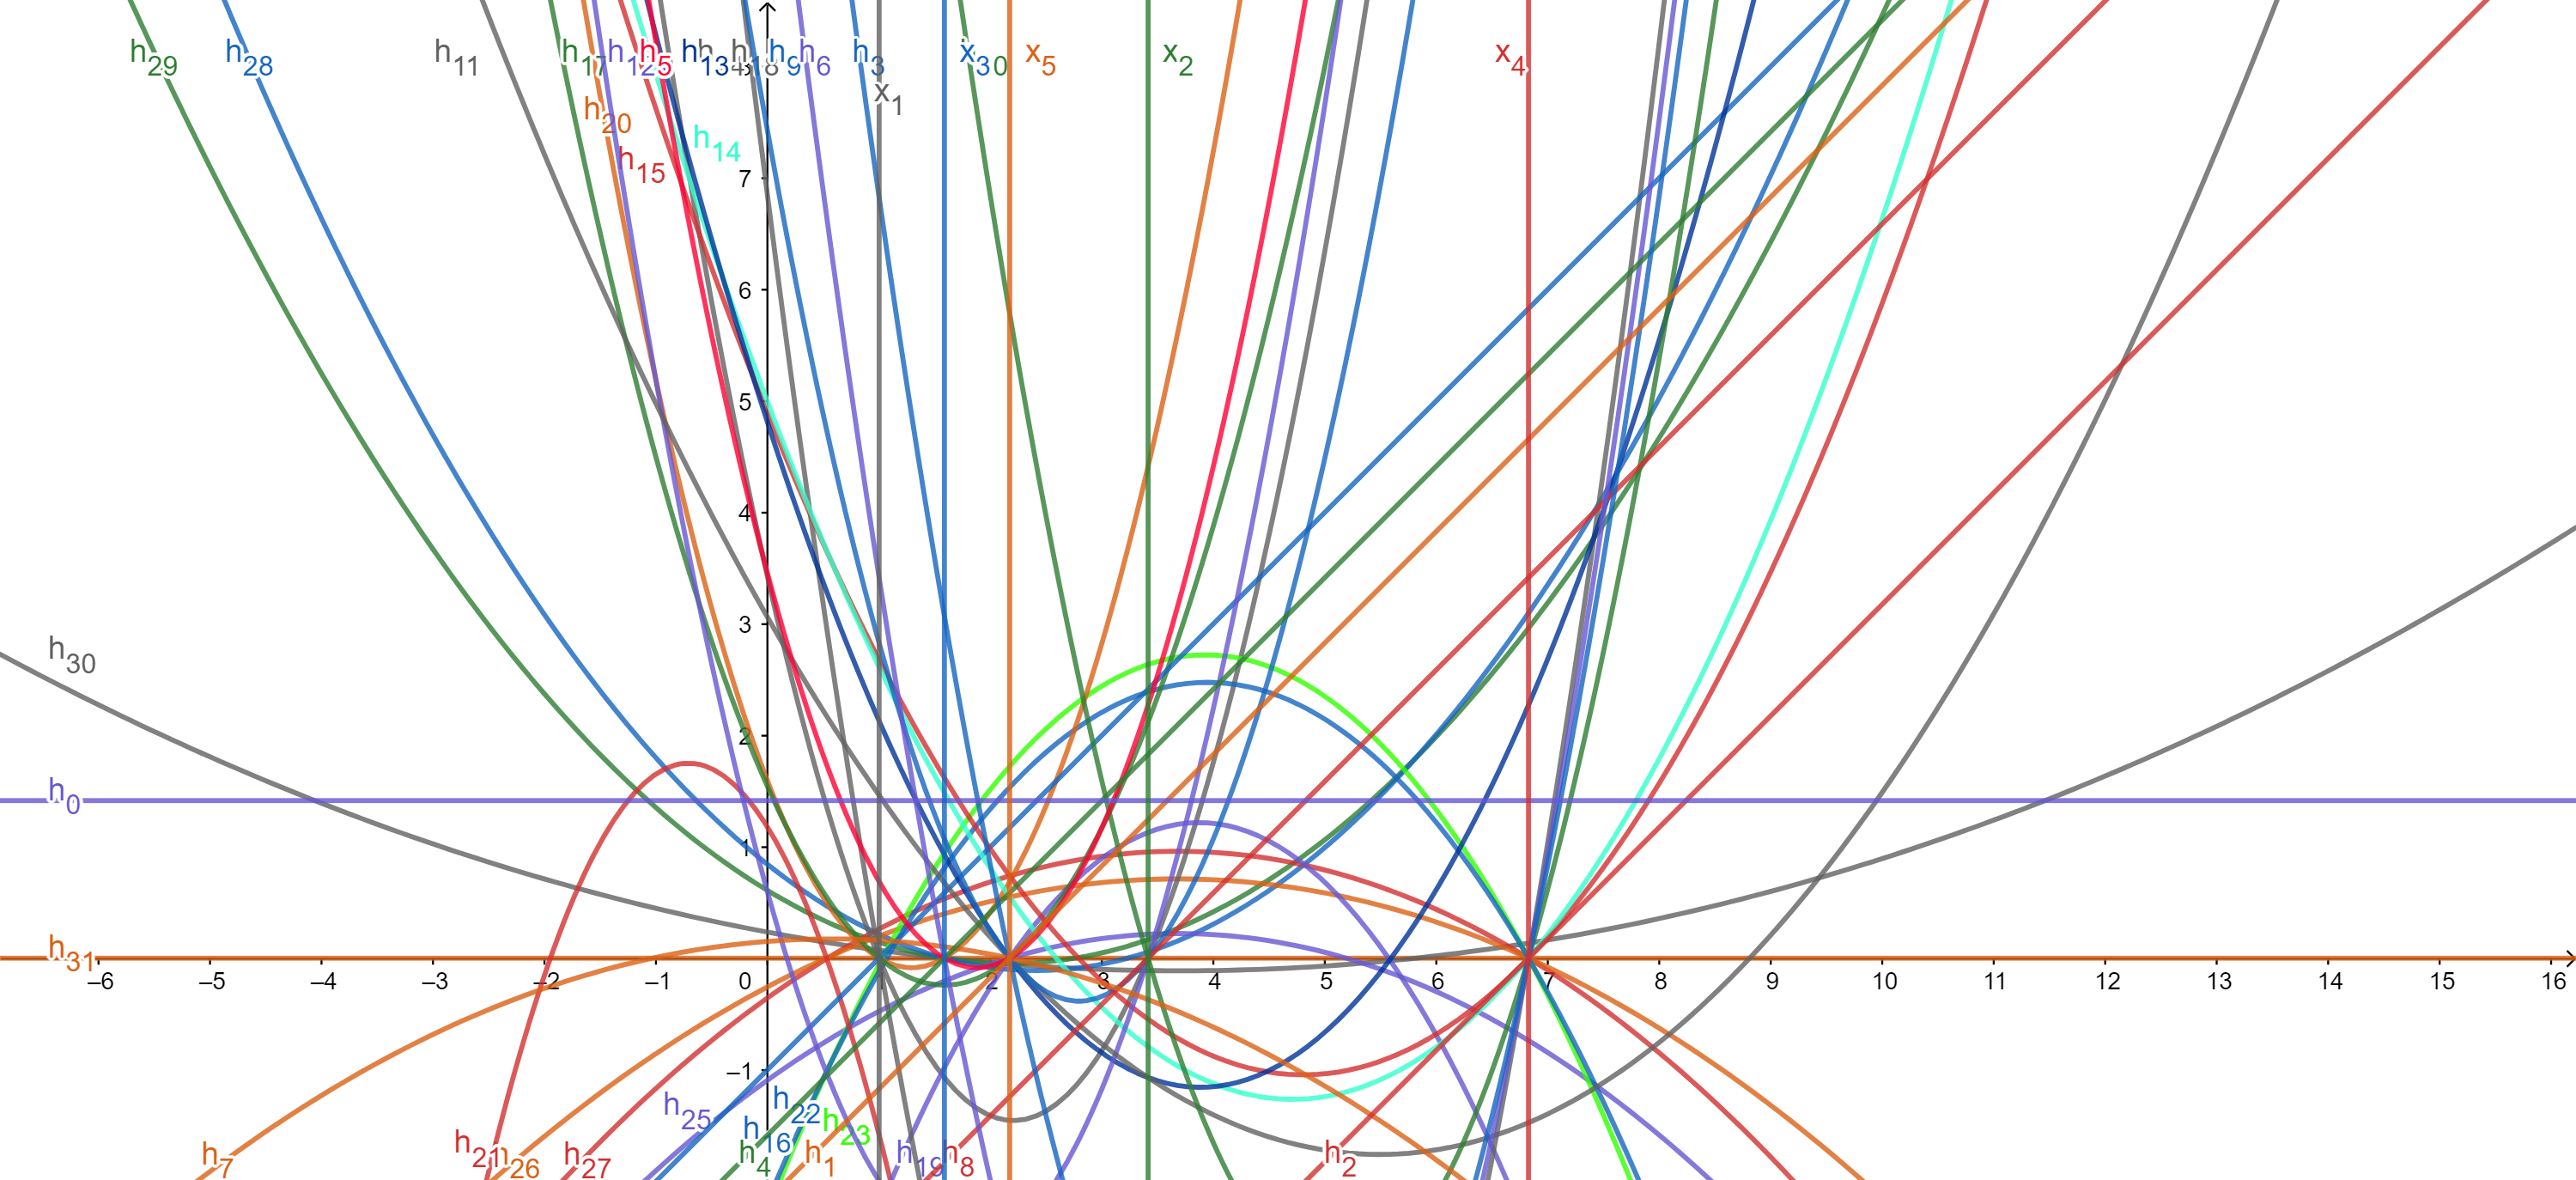
\includegraphics[width = 1 \linewidth]{geogebra-export (4).png}
        \caption{The case $n=2$, with $32$ polynomials and 5 variables}
        \label{fig:my_label}
\end{figure}
    \end{itemize}
\end{frame}
\begin{frame}{Proof that when $n=2$, $VCDim(\mathcal{H}) \leq 5$}
    \begin{itemize}
        \item We now show 6 points cannot be shattered
        \pause
        \vskip.35in
        \item Suppose there exists 6 points $x_1,x_2,\cdots,x_6$ such that $\mathcal{H}$ shatters them. Let $f_1,f_2,\cdots,f_6$ be polynomials of degree at most $2$ such that
        $$f_i(x_j) \not \in \mathbb{Q} \text{ if and only if } i = j$$
        \pause
        \vskip.25in
        \item Consider the value of $f_1(x_1),f_1(x_2),\cdots,f_1(x_6)$. Among the 5 numbers $f_1(x_2),f_1(x_3),f_1(x_4),f_1(x_5), f_1(x_6)$, $3$ cannot be the same. 
        
    \end{itemize}
\end{frame}
\begin{frame}{Proof that when $n=2$, $VCDim(\mathcal{H}) \leq 5$ (Continued)}
    \begin{itemize}
        \item WLOG, suppose $f_1(x_6) \neq f_1(x_1),f_1(x_2),\cdots,f_1(x_4)$. Let
        $$I=\{1,2,5 \},J=\{2,3,4 \}$$
        \pause
        \vskip.2in
        \item Define $A(i,j)=f_i(x_6)-f_i(x_j)$ with $f_i(x) = a_ix^2+b_ix+c_i$. 
        \pause
        \vskip.2in
        \item Then $A(1,j) \neq 0 \ \forall \ j \in J$ and
        $$\frac{A(i,j)}{A(1,j)}=\frac{a_i(x_6+x_j)+b_i}{a_1(x_6+x_j)+b_1}$$
        is irrational if and only if $(i,j) \neq (2,2)$
    \end{itemize}
\end{frame}
\begin{frame}{Proof that when $n=2$, $VCDim(\mathcal{H}) \leq 5$ (Continued)}
    \begin{itemize}
        \item Now, for $i \in \{2,5\}$ and $j \in \{2,3\}$, we have
        \begin{align*}
            \frac{A(i,j)}{A(1,j)}-\frac{A(i,4)}{A(1,4)}&=\frac{(x_4-x_j)(b_ia_1-b_1a_i)}{(a_1(x_6+x_j)+b_1)(a_1(x_6+x_4)+b_1)}
        \end{align*}
        \pause
        \vskip.1in
        \item Now if $j=2$, we have when $(i,j)=(2,2), \frac{(x_4-x_2)(b_2a_1-b_1a_2)}{(a_1(x_6+x_2)+b_1)(a_1(x_6+x_4)+b_1)} \not \in \mathbb{Q}$ and if $(i,j)=(5,2)$, $\frac{(x_4-x_2)(b_5a_1-b_1a_5)}{(a_1(x_6+x_2)+b_1)(a_1(x_6+x_4)+b_1)} \in \mathbb{Q}$
        \pause
        \vskip.1in
        \item If $b_1a_5=a_1b_5$, there must be 2 constants $u,v$ such that $f_5(x)=uf_1(x)+v$. Then plug in $x=x_6$ and $x=x_2$, we have
        $$u=\frac{f_5(x_6)-f_5(x_2)}{f_1(x_6)-f_1(x_2)} \in \mathbb{Q}$$
        \pause
        \vskip.1in
        \item On the other hand, if we plug in $x=x_1,x=x_k \neq x_5$ such that $f_5(x_1) \neq f_5(x_k)$ (Which is possible as above). Then
        $$u=\frac{f_5(x_k)-f_5(x_1)}{f_1(x_k)-f_1(x_1)} \not \in \mathbb{Q}$$
        which is clearly impossible
    \end{itemize}
\end{frame}
\begin{frame}{Prove that when $n=2$, $VCDim(\mathcal{H}) \leq 5$ (Continue)}
    \begin{itemize}
        \item Hence, we have $b_1a_5 \neq b_5a_1$. Therefore, $\frac{b_5a_1-b_1a_5}{b_2a_1-b_1a_2} \not \in \mathbb{Q}$.
        \pause
        \vskip.3in
        \item Now if $j=3$, with similar arguments as above, $\frac{b_5a_1-b_1a_5}{b_2a_1-b_1a_2} \in \mathbb{Q}$, which is a contradiction
        \pause
        \vskip.3in
        \item In conclusion, $VCDim(\mathcal{H}) \leq 5$. As proven above, $VCDim(\mathcal{H}) \geq 5$.
        \pause
        \vskip.3in
        \item As a result, we must have $VCDim(\mathcal{H})=5$ (Q.E.D)
    \end{itemize}
\end{frame}
\subsection{General case}
\begin{frame}{Future approaches}
    \begin{itemize}
        \item Using a similar argument, we may be able to extend this to the general case. We are still trying to work through it all.\\
        \pause
        \vskip.4in
        \item For the upper bound, we have found that a set of $2n+2$ algebraic numbers cannot be shattered. Transcendental numbers will be considered after.\\
        \pause
        \vskip.4in
        \item We hope to generalize the results from $\mathbb{R}$ and $\mathbb{Q}$ to more general fields $F' \subseteq F$
    \end{itemize}
\end{frame}
% % \begin{frame}{Prove $VCDim(\mathcal{H}) \geq 2\dim{F}-1$}
% %     \begin{itemize}
% %     \item We will show by induction on the dimension of $F$. For $\dim F=1/2/3$, the idea is proven above
% %     \pause
% %     \item Suppose for the case $dim \ F =n+1$, or $f(x)$ is a polynomial with degree less than or equal to $n$, there exists a real set $S=\{x_1,x_2,\cdots,x_{2n+1} \}$ of $2n+1$ elements such that $\mathcal{H}$ shatters $S$
% %     \pause
% %     \item We will show that if we increase the degree of $f$ by $1$, we can have 2 additional numbers $u$,$v$ such that when add in $S$, $\mathcal{H}$ will shater it. Consider $4$ cases
% %     \pause
% %     \item Case 1: Suppose for some $f$, we need $f(u) \not \in \mathbb{Q}$, $f(v) \not \in \mathbb{Q}$, then $S$ can shattered any set with less than or equal to $2n+1+2-2=2n+1$ elements, which is proved above
% %     \pause
% %     \item Case 2: Suppose for some $f$, we need $f(u) \not \in \mathbb{Q},f(v) \in \mathbb{Q}$. If among the first $2n+1$ numbers, there is a number $x_J$ such that $f(x_j) \not \in \mathbb{Q}$. We take the polynomial $k(x)$ that gives the condition for the first $2n+1$ points. Then $deg(k) \leq n$. Then if we take $f(x)=k(x)(x-v)$. We need to consider 
% %     \end{itemize}
% % \end{frame}
% \begin{frame}{Main result: Proof that $VCDim(\mathcal{H}) \geq 2\dim{F}-1$}
%     \begin{itemize}
%         \item We define the sequence $(x_i)$ to be
%     $$\begin{cases}
%     x_i = i+2^{i-2}\sqrt{2} & \forall 2 \leq i \leq 2n+1\\
%     x_1 = 1
%     \end{cases}$$. We will show that $\mathcal{H}$ will shatter this set by induction\\
%     \pause
%     \item For $n=1,2$, we have proved above. Suppose the claim is true for $n=k$, then we will have the set
%     $$S=\{1,2+\sqrt{2},3-\sqrt{2},\cdots,2k+k\sqrt{2},2k+1-k\sqrt{2}\}$$
%     will be shattered by $\mathcal{H}$
%     \pause
%     \item We will prove that if we add in $x_{2k+2}=2k+2+(k+1)\sqrt{2},x_{2k+3}=2k+3-(k+1)\sqrt{2}$, then the claim is still true. It is easy to consider the case whether it can shatter a set with at most $n+1$ points.\\
%     \pause
%     \item In fact, we just need to look at the case that there exists $2n+2$ polynomials $f_1,\cdots,f_{2k+3}$ such that
%     $$f_i(x_i) \not \in \mathbb{Q} \ \forall 1 \leq i \leq 2k+3, f_i(x_i) \not \in \mathbb{Q} \ \forall 1 \leq i \neq j \leq 2k+3$$
%     \end{itemize}
    
% \end{frame}
% \begin{frame}{$VCDim(\mathcal{H}) \geq 2\dim{F}-1$ (Continue)}
%     \begin{itemize}
%         \item If $i=2k+3$ or $i=2k+2$, WLOG, let $i=2k+3$, the other case will be the same
%         $$f(x) = (x-x_{2k+2})(a_1f_1+a_2f_2+\cdots+a_{2k+1}f_{2k+1})$$
%         With $f_i$ be a n-degree polynomial from the claim of $n=k$.
%         \pause
%         \item Then for any $1 \leq j \leq 2k+1$, we need
%         $$f(x_j) \in \mathbb{Q} \iff (x_j-x_i)(a_1f_1(x_j)+a_2f_2(x_j)+\cdots+a_{2k+1}f_{2k+1}(x_j)) \in \mathbb{Q}$$
%         with each $a_i = u_i+v_i \sqrt{2}, u_i,v_i \in \mathbb{Q}$.\\
%         \pause
%         \item Suppose $f_i(x_{i+1})=0$ for any $1 \leq i \leq 2k+1$, with the fact that $f_{2k+1}(x_1)=1$. Let $x=x_j$, we will have
%         $$(x_j-x_{2k+2})(a_1f_1(x_{j})+a_2f_2(x_j)+\cdots+a_{j-2}f_{j-2}(x_j)+a_jf_j(x_j)+\cdots+a_{2k+1}f_{2k+1}(x_j)) \in \mathbb{Q}$$
%         $$\iff(x_j-x_{2k+2})((u_1+v_1\sqrt{2})q_{1j}+(u_2+v_2\sqrt{2})q_{2j}+\cdots+$$
%     \end{itemize}
% \end{frame}

\begin{frame}{Reference}
    \begin{thebibliography}{3}

%\bibitem{Falc85} K. Falconer, {\it On the Hausdorff dimensions of distance sets}, Mathematika, \textbf{32}, no.2, 206-212 (1985). 

\bibitem{DS14} S. Shalev-Shwartz and S. Ben-David, {\it Understanding Machine Learning: From Theory to Algorithms}, Cambridge University Press, (2014). 
\vskip.2in
\bibitem{DS14} Noga Alon and Joel H. Spencer, {\it The Probabilistic Method}, Wiley Publishing, (2016). 


\end{thebibliography} 
\end{frame}


% \frame{\myframetitle{References}


% \begin{thebibliography}{8}

% \bibitem{} D. Covert, {\it The Finite Field Distance Problem}, MAA Press, an imprint of the American Mathematical Society, (2021).

% \vskip.15in

% \bibitem{} A. Iosevich and H. Parshall, {\it Embedding distance graphs in finite field vector spaces}, (2018).

% \vskip.15in

% \bibitem{} A. Iosevich, G. Jardine and B. McDonald, {\it Cycles of arbitrary length in distance graphs on $\mathbb{F}_q^d$}, (2021).

% \end{thebibliography} 


% }

\begin{frame}{Thanks!}
    \begin{itemize}
        \item We would like to thank our project supervisors for their wonderful help and support during the research. We are looking forward to continuing our work with them in the future.
        \pause
        \vskip.5in
        
        \item Special thanks to NSF for providing our groups with funding.
    \end{itemize}
\end{frame}
\end{document}
